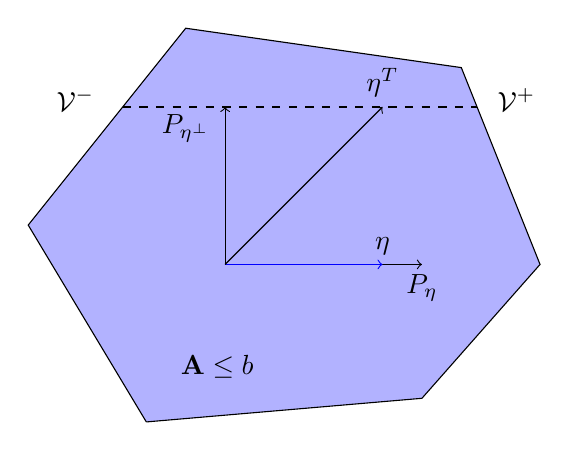
\begin{tikzpicture}
\draw (-1,-2) -- (-2.5,0.5) -- (-0.5,3)-- (3,2.5) -- (4,0) -- (2.5,-1.7) -- (-1,-2)[fill = blue!30];
\draw [<-] (0,2) node [label={[xshift=-0.5cm, yshift=-0.7cm]$P_{\boldsymbol{\eta}^\perp} \y$}] {} -- (0,0);
\draw[<-] (2.5,0) node [below] {$P_{\boldsymbol{\eta}} \y$} -- (0,0);
\draw[<-][blue] (2,0) node [black, above] {$\boldsymbol{\eta}$} -- (0,0);
\draw[<-] (2,2) node [above] {$\boldsymbol{\eta}^T \y$} -- (0,0) node [label={[xshift=1.7cm, yshift=1cm]$\y$}] {};
\draw[dashed] (-1.3,2) node [label={[xshift=-0.6cm, yshift=-0.3cm]$\mathcal{V}^- \del{\y}$}] {} -- (3.2,2) node [label={[xshift=0.5cm, yshift=-0.3cm]$\mathcal{V}^+ \del{\y}$}] {};
\draw node [label={[xshift=-0.1cm, yshift=-1.7cm]$\cbr{\mathbf{A} \y \leq b}$}] {};
\end{tikzpicture}